\documentclass[12pt]{article}
\usepackage{graphicx}
\usepackage[a4paper, margin=1in]{geometry}
\usepackage{amsmath}
\usepackage[utf8]{inputenc}
\usepackage{listings}
\usepackage{xcolor}

\usepackage{amsfonts}
\usepackage{amssymb}
\usepackage{geometry}
\usepackage{titlesec}
\usepackage{fancyhdr}
\usepackage{lipsum}


\lstdefinestyle{mystyle}{
    backgroundcolor=\color{white},
    commentstyle=\color{codegreen},
    keywordstyle=\color{magenta},
    numberstyle=\tiny\color{codegray},
    stringstyle=\color{codepurple},
    basicstyle=\ttfamily\footnotesize,
    breakatwhitespace=false,
    breaklines=true,
    captionpos=b,
    keepspaces=true,
    numbers=left,
    numbersep=5pt,
    showspaces=false,
    showstringspaces=false,
    showtabs=false,
    tabsize=2
}

\lstset{style=mystyle}
\renewcommand{\baselinestretch}{1.3}

\definecolor{codegreen}{rgb}{0,0.6,0}
\definecolor{codegray}{rgb}{0.5,0.5,0.5}
\definecolor{codepurple}{rgb}{0.58,0,0.82}

% Configuración de página
\geometry{a4paper, margin=1in}
\pagestyle{fancy}
\fancyhf{}
\rhead{Eidan Owen Plata Salinas}
\lhead{Cadenas Ocultas de Markov}
\cfoot{\thepage}

% Títulos
\titleformat{\section}[block]{\normalfont\Large\bfseries}{\thesection}{1em}{}
\titlespacing*{\section}{0pt}{\baselineskip}{\baselineskip}

% Metadatos
\title{Clasificación con Cadenas Ocultas de Markov: Implementacion y comparación}
\author{Eidan Owen Plata Salinas}
\date{\today}



\begin{document}
\maketitle
\pagebreak



\section*{Marco teórico}

Las cadenas ocultas de Markov (HMM) son una clase de modelos estadísticos
ampliamente utilizados en una variedad de aplicaciones, desde el
procesamiento del lenguaje natural hasta la bioinformática y la ingeniería de
señales. Estos modelos se basan en la teoría de las cadenas de Markov, pero
incorporan una capa de ocultamiento que los hace especialmente adecuados
para modelar secuencias de datos observados en los que la estructura
subyacente es desconocida o no directamente observable.\vspace{1cm}


Las cadenas ocultas de Markov se componen de tres componentes clave: los
estados ocultos, las observaciones y las probabilidades de transición. Los
estados ocultos representan la estructura subyacente del sistema que estamos
tratando de modelar. Cada estado oculto tiene una distribución de probabilidad
asociada que describe la probabilidad de emitir una observación dada cuando
el sistema se encuentra en ese estado. Además, las HMM incluyen
probabilidades de transición que indican cómo los estados ocultos evolucionan
con el tiempo. Estas probabilidades pueden ser representadas mediante
matrices de transición.\vspace{1cm}


El proceso de entrenar una cadena oculta de Markov implica estimar los
parámetros desconocidos, es decir, las probabilidades de emisión y transición,
a partir de datos observados. Uno de los algoritmos más utilizados para este
propósito es el algoritmo de Baum-Welch, que utiliza el algoritmo de
expectativa-maximización (EM) para encontrar los valores óptimos de los
parámetros. El algoritmo de Viterbi, por otro lado, se utiliza para encontrar la
secuencia de estados ocultos más probable dadas las observaciones.\vspace{1cm}


Las cadenas ocultas de Markov han encontrado aplicaciones en una amplia
gama de campos. En el procesamiento del lenguaje natural, se utilizan para
modelar la estructura gramatical de las oraciones y la predicción de palabras
en la escritura automática. En bioinformática, son esenciales para el análisis
de secuencias de ADN y proteínas, así como para la predicción de estructuras
secundarias de proteínas. En la ingeniería de señales, las HMM se utilizan en
reconocimiento de voz, procesamiento de señales de audio y más.\vspace{1cm}


La elección del método de aprendizaje de máquina adecuado depende en gran
medida de la naturaleza de los datos y la tarea específica que se debe abordar.
Las cadenas ocultas de Markov son poderosas para modelar secuencias de
datos con estructuras ocultas y dependencias temporales, pero no son la
elección óptima para todos los problemas. k-NN, Regresión Logística, SVM y
Clasificadores Bayesianos son métodos sólidos que funcionan bien en
diferentes contextos, y su selección debe basarse en la comprensión de los
datos y los objetivos de la tarea.\vspace{1cm}


Las HMM y k-NN son enfoques diferentes para abordar problemas de
clasificación. Las HMM se centran en modelar secuencias de datos y son
particularmente útiles cuando se trata de datos secuenciales, como el
procesamiento del lenguaje natural o el análisis de señales de tiempo. Por otro
lado, k-NN se basa en la similitud de características y es efectivo en problemas
de clasificación no secuenciales. La elección entre HMM y k-NN depende de la
naturaleza de los datos y la tarea específica.\vspace{1cm}


La Regresión Logística es un método de clasificación ampliamente utilizado
que modela relaciones lineales entre características y la probabilidad de
pertenecer a una clase. A diferencia de las HMM, que son más adecuadas para
datos secuenciales, la Regresión Logística se aplica principalmente a datos
tabulares y categóricos. Las HMM son más flexibles cuando se trata de
modelar secuencias temporales y dependencias ocultas entre observaciones.\vspace{1cm}


Las SVM son conocidas por su eficacia en la clasificación de datos lineal y no
lineal. Mientras que las HMM se centran en secuencias, las SVM son ideales
para problemas de clasificación binaria o multiclase en datos de alta
dimensión. La elección entre HMM y SVM depende de si se trata de datos
secuenciales y si se requiere una separación de hiperplano eficiente.\vspace{1cm}


Los Clasificadores Bayesianos se basan en el teorema de Bayes y utilizan
distribuciones de probabilidad para modelar la probabilidad condicional de
pertenecer a una clase dada un conjunto de características observadas.
Aunque ambos HMM y los Clasificadores Bayesianos se basan en
probabilidades, los HMM incorporan la noción de estados ocultos y transiciones
de estado, lo que los hace más adecuados para modelar secuencias
temporales y datos con estructuras ocultas.\vspace{1cm}





\vspace{1cm}

\section*{Explicacion por funciones}
\vspace{1cm}
\subsection*{Funcion \texttt{cargar datos}}



\vspace{1cm}

\begin{lstlisting}[language=Python]
def cargar_datos(ruta_csv):
	data = pd.read_csv(ruta_csv, header=None)
	X = data.iloc[:, :-1].values
	y = data.iloc[:, -1].values
	return X, y


\end{lstlisting}
\vspace{1cm}

Esta función surge de la necesidad de cargar y procesar conjuntos de datos almacenados en archivos CSV (Valores Separados por Comas), un formato ampliamente utilizado para almacenar datos en forma tabular. es un paso crítico, ya que los modelos necesitan datos en un formato adecuado para poder entrenarlos y hacer predicciones.\vspace{1cm}

Funciona leyendo un archivo CSV desde la ubicación especificada por ruta\_csv. Utiliza la biblioteca pandas, una herramienta poderosa en Python para la manipulación de datos, para leer el archivo. Dentro de la función, pd.read\_csv(ruta\_csv, header=None) lee el archivo CSV sin asumir ninguna fila de encabezado. Esto resulta en un DataFrame de Pandas, una estructura de datos bidimensional, donde las columnas y filas se identifican por números enteros comenzando desde 0. Luego, la función separa este DataFrame en dos partes: X y y. X contiene todas las columnas excepto la última, asumiendo que estas son las características (o atributos) del conjunto de datos. Por otro lado, y contiene solo la última columna, asumiendo que esta es la variable objetivo o las etiquetas que se quieren predecir.\vspace{1cm}

Actúa como el punto de entrada para los datos que se utilizarán en todo el proceso de aprendizaje automático. Sin una correcta carga y separación de las características y las etiquetas, los pasos subsiguientes, como el entrenamiento y la evaluación de modelos, no podrían llevarse a cabo correctamente. Esta función asegura que los datos estén en el formato adecuado y disponibles para ser procesados y utilizados en las fases de entrenamiento y validación de los diferentes modelos de clasificación implementados en el código.

\vspace{1cm}

\subsection*{Funcion \texttt{cargar\_datos\_markov}}
\vspace{1cm}

\begin{lstlisting}[language=Python]

def cargar_datos_markov(filename):
	columns = ['', '', '', '', '', '', '']
	data = pd.read_csv(filename, header=None, names=columns)
	label_encoder = LabelEncoder()
	data['label'] = label_encoder.fit_transform(data['label'])
	return data, label_encoder

\end{lstlisting}
\vspace{1cm}

La función cargar\_datos\_markov comienza leyendo un archivo CSV utilizando pd.read\_csv, similar a cargar\_datos. Sin embargo, aquí se especifican nombres de columnas con names=columns, porque el archivo CSV, extraido del repositorio para machine learning, no tiene una fila de encabezado y cada columna en el archivo se corresponde con un nombre específico en la lista columns. Esta característica es crucial para el procesamiento posterior, especialmente en aplicaciones que utilizan modelos de Markov, donde cada columna puede representar diferentes aspectos de los datos, como coordenadas espaciales o temporales y etiquetas de clasificación. Después de leer los datos, la función emplea LabelEncoder de la biblioteca sklearn para transformar las etiquetas categóricas en representaciones numéricas, un paso necesario para la mayoría de los algoritmos de aprendizaje automático que requieren entradas numéricas.\vspace{1cm}

El papel de esta función en el código es doble. Primero, prepara el conjunto de datos para ser utilizado con modelos específicos de HMM. Los modelos HMM son particularmente sensibles a la forma en que se presentan los datos, por lo que asegurarse de que los datos estén correctamente formateados y codificados es crucial para el éxito del modelado. Segundo, la función establece un puente entre la representación cruda de los datos (a menudo en forma de texto o categorías en un archivo CSV) y una representación numérica que puede ser procesada para los algoritmos.

\vspace{1cm}

\subsection*{Función \texttt{separar\_datos\_markov}}
\vspace{1cm}

\begin{lstlisting}[language=Python]

def separar_datos_markov(data):
	X = data[['', '', '', '', '', '']]
	y = data['label']
	return train_test_split(X, y, test_size=0.3, random_state=42)

\end{lstlisting}
\vspace{1cm}

La función toma un DataFrame data como entrada, que ya ha sido procesado por la función cargar\_datos\_markov. Esta entrada incluye varias columnas de características sin nombre y una columna de etiquetas ('label'). La función separar\_datos\_markov separa estas características y etiquetas en dos conjuntos distintos, X y y, respectivamente. Esto es estándar en el flujo de trabajo de aprendizaje automático, donde X representa los datos de entrada que se utilizan para el entrenamiento y la predicción, y y representa las etiquetas o los resultados que se deben predecir. Luego, emplea la función train\_test\_split de sklearn.model\_selection para dividir estos conjuntos de datos en subconjuntos de entrenamiento y prueba. Esta división es crucial para validar el rendimiento del modelo: el modelo se entrena en un conjunto de datos y luego se prueba en un conjunto separado para evaluar su capacidad de generalizar a datos no vistos.\vspace{1cm}

El papel de separar\_datos\_markov en el código es preparar el escenario para el entrenamiento y la validación eficaces de los modelos de HMM. Al separar los datos en conjuntos de entrenamiento y prueba, permite una evaluación imparcial del modelo. La elección de las características (X) y las etiquetas (y), así como su posterior división en conjuntos de entrenamiento y prueba, son pasos fundamentales en cualquier flujo de trabajo de modelado predictivo. La función garantiza que los datos estén correctamente organizados y divididos antes de proceder con el entrenamiento y la evaluación de modelos.

\vspace{1cm}

\subsection*{Función \texttt{entrenar\_markov}}
\vspace{1cm}

\begin{lstlisting}[language=Python]
def entrenar_markov(X_train, y_train):
	hmms = {}
	for label in y_train.unique():
		model = hmm.GaussianHMM(n_components=4, covariance_type="diag", n_iter=100)
		model.fit(X_train[y_train == label])
		hmms[label] = model
	return hmms

\end{lstlisting}
\vspace{1cm}

La función toma dos argumentos: X\_train y y\_train. Estos representan los conjuntos de datos de entrenamiento, donde X\_train contiene las características (datos de entrada) y y\_train contiene las etiquetas correspondientes. La función itera sobre las etiquetas únicas en y\_train, entrenando un modelo HMM para cada etiqueta. Utiliza hmm.GaussianHMM de la biblioteca hmmlearn, que implementa un modelo HMM con emisiones gaussianas. Para cada etiqueta única, selecciona las filas de X\_train que corresponden a esa etiqueta y entrena un modelo HMM en estos datos. El modelo HMM se configura con un número específico de componentes (estados ocultos) y un tipo de covarianza, y se entrena hasta un número máximo de iteraciones. Esto resulta en un conjunto de modelos HMM, uno para cada etiqueta, almacenados en el diccionario hmms.\vspace{1cm}


Dado que los modelos de HMM son especialmente adecuados para datos secuenciales o temporales, esta función permite al usuario aplicar este enfoque avanzado de modelado a conjuntos de datos relevantes. Al entrenar un modelo HMM específico para cada etiqueta, la función se adapta a la naturaleza de los datos y las peculiaridades de cada clase o categoría en el conjunto de datos. Esto es particularmente útil en aplicaciones como el reconocimiento de patrones, el análisis de series temporales o el procesamiento del lenguaje natural, donde la relación entre las secuencias de datos y los estados ocultos o las etiquetas es compleja.

\vspace{1cm}

\subsection*{Función \texttt{entrenar\_markov}}
\vspace{1cm}

\begin{lstlisting}[language=Python]
	def entrenar_markov(X_train, y_train):
	hmms = {}
	for label in y_train.unique():
	model = hmm.GaussianHMM(n_components=4, covariance_type="diag", n_iter=100)
	model.fit(X_train[y_train == label])
	hmms[label] = model
	return hmms
	
\end{lstlisting}
\vspace{1cm}

La función toma dos argumentos: X\_train y y\_train. Estos representan los conjuntos de datos de entrenamiento, donde X\_train contiene las características (datos de entrada) y y\_train contiene las etiquetas correspondientes. La función itera sobre las etiquetas únicas en y\_train, entrenando un modelo HMM para cada etiqueta. Utiliza hmm.GaussianHMM de la biblioteca hmmlearn, que implementa un modelo HMM con emisiones gaussianas. Para cada etiqueta única, selecciona las filas de X\_train que corresponden a esa etiqueta y entrena un modelo HMM en estos datos. El modelo HMM se configura con un número específico de componentes (estados ocultos) y un tipo de covarianza, y se entrena hasta un número máximo de iteraciones. Esto resulta en un conjunto de modelos HMM, uno para cada etiqueta, almacenados en el diccionario hmms.\vspace{1cm}


Dado que los modelos de HMM son especialmente adecuados para datos secuenciales o temporales, esta función permite al usuario aplicar este enfoque avanzado de modelado a conjuntos de datos relevantes. Al entrenar un modelo HMM específico para cada etiqueta, la función se adapta a la naturaleza de los datos y las peculiaridades de cada clase o categoría en el conjunto de datos. Esto es particularmente útil en aplicaciones como el reconocimiento de patrones, el análisis de series temporales o el procesamiento del lenguaje natural, donde la relación entre las secuencias de datos y los estados ocultos o las etiquetas es compleja.

\vspace{1cm}

\subsection*{Función \texttt{clasificar\_markov}}
\vspace{1cm}

\begin{lstlisting}[language=Python]
def clasificar_markov(X_test, hmms) -> list:
	predictions = []
	for index, row in X_test.iterrows():
		max_score = float('-inf')
		best_label = None
		for label, model in hmms.items():
			score = model.score(row.to_frame().T)
			if score > max_score:
				max_score = score
				best_label = label
			predictions.append(best_label)
	return predictions
	
\end{lstlisting}
\vspace{1cm}

La función clasificar\_markov(X\_test, hmms) toma dos argumentos: X\_test, que es un conjunto de datos de prueba, y hmms, un diccionario de modelos HMM entrenados, donde cada clave corresponde a una etiqueta de clase única. El propósito principal de esta función es iterar a través de cada muestra en X\_test y asignarle la etiqueta de clase más probable basada en los modelos HMM.\vspace{1cm}


Dentro de la función, se itera sobre cada fila (ejemplo) en X\_test. Para cada ejemplo, la función calcula el 'score' de cada modelo HMM en hmms. Este 'score' representa la probabilidad logarítmica de que el modelo HMM genere la secuencia observada. La función identifica el modelo que da el máximo 'score' para esa fila particular. La clave (etiqueta de clase) de este modelo HMM con el 'score' más alto se selecciona como la etiqueta predicha para la muestra actual.\vspace{1cm}

Después de procesar todas las filas en X\_test, la función acumula todas las etiquetas predichas en una lista predictions. Esta lista de predicciones se devuelve como resultado de la función. En resumen, clasificar\_markov aplica modelos HMM a un conjunto de datos de prueba para predecir la clase de cada muestra, basándose en la probabilidad logarítmica de que cada modelo HMM genere la secuencia observada en los datos de prueba.

\vspace{1cm}

\subsection*{Función \texttt{validacion\_cruzada\_kfold}}
\vspace{1cm}

\begin{lstlisting}[language=Python]
def validacion_cruzada_kfold(data, k):
	kf = KFold(n_splits=k, shuffle=True, random_state=42)
	scores = []
	
	for train_index, test_index in kf.split(data):
		X_train, X_test = data.iloc[train_index], data.iloc[test_index]
		y_train, y_test = X_train['label'], X_test['label']
		X_train = X_train.drop('label', axis=1)
		X_test = X_test.drop('label', axis=1)
		
		hmms = entrenar_markov(X_train, y_train)
		predictions = clasificar_markov(X_test, hmms)
		score = evaluar_markov(predictions, y_test)
		scores.append(score)
	
	return sum(scores) / len(scores)
	
\end{lstlisting}
\vspace{1cm}

La función  acepta dos argumentos: data, que es el conjunto de datos completo, y k, que es el número de particiones (folds) a crear para la validación cruzada. El propósito de esta función es evaluar de manera más robusta el rendimiento de los modelos HMM al dividir el conjunto de datos en k partes, entrenando el modelo en k-1 de estas partes y validándolo en la parte restante. Este proceso se repite k veces, con cada parte siendo utilizada exactamente una vez como conjunto de prueba.\vspace{1cm}

Dentro de la función, se utiliza el objeto KFold de sklearn para generar índices de particiones de entrenamiento y prueba. Para cada partición, se separan los datos en conjuntos de entrenamiento y prueba. Luego, se llama a la función entrenar\_markov para entrenar modelos HMM con los datos de entrenamiento, y se utiliza la función clasificar\_markov para predecir las etiquetas de los datos de prueba. Después de esto, se evalúa el rendimiento de las predicciones usando la función evaluar\_markov, que compara las predicciones con las etiquetas reales del conjunto de prueba.

\vspace{1cm}

\subsection*{Función \texttt{puntaje\_markov}}
\vspace{1cm}

\begin{lstlisting}[language=Python]
def puntaje_markov(archivo):
	data, label_encoder = cargar_datos_markov(archivo)
	accuracy_promedio = validacion_cruzada_kfold(data, 5)
	return accuracy_promedio
	
\end{lstlisting}
\vspace{1cm}

La función comienza cargando el conjunto de datos desde un archivo CSV usando la función cargar\_datos\_markov(archivo). Esta función no solo carga los datos, sino que también realiza una codificación de las etiquetas (o clases) mediante LabelEncoder. Esto es necesario porque los modelos HMM generalmente requieren que las etiquetas de salida estén en un formato numérico. El archivo CSV que se pasa como argumento a puntaje\_markov contiene los datos que se usarán para entrenar y probar los modelos HMM.\vspace{1cm}

Después de cargar y preparar los datos, la función puntaje\_markov procede a evaluar el rendimiento de los modelos HMM utilizando la técnica de validación cruzada K-Fold. Para esto, llama a la función validacion\_cruzada\_kfold(data, 5), pasando los datos y el número de particiones (en este caso, 5). La función de validación cruzada K-Fold divide el conjunto de datos en 5 partes, entrenando el modelo en 4 de estas partes y validándolo en la parte restante en cada iteración. Esto ayuda a asegurar que la evaluación del modelo sea robusta y menos propensa a sesgos debido a la partición particular de los datos.\vspace{1cm}

La función validacion\_cruzada\_kfold retorna un puntaje de precisión promedio obtenido a través de todas las iteraciones de la validación cruzada. Este puntaje es una métrica clave que indica qué tan bien el modelo HMM está realizando predicciones en los conjuntos de datos de prueba. La función puntaje\_markov luego devuelve este puntaje de precisión promedio como su resultado final.


\vspace{1cm}

\subsection*{Función \texttt{k\_fold\_cross\_validation}}
\vspace{1cm}

\begin{lstlisting}[language=Python]
def k_fold_cross_validation(X, y, k, modelo):
	fold_size = len(X) // k
	indices = np.arange(len(X))
	np.random.shuffle(indices)
	scores = []
	
	for fold in range(k):
	test_indices = indices[fold * fold_size : (fold + 1) * fold_size]
	train_indices = np.setdiff1d(indices, test_indices)
	
	
	X_train, X_test = X[train_indices], X[test_indices]
	y_train, y_test = y[train_indices], y[test_indices]
	
	
	modelo_clonado = clone(modelo)
	modelo_clonado.fit(X_train, y_train)
	
	
	y_pred = modelo_clonado.predict(X_test)
	score = accuracy_score(y_test, y_pred)
	scores.append(score)
	
	return scores
	
\end{lstlisting}
\vspace{1cm}

La función k\_fold\_cross\_validation(X, y, k, modelo) toma cuatro argumentos: X y y, que son los conjuntos de características y etiquetas respectivamente, k que es el número de particiones para la validación cruzada, y modelo, que es el modelo de aprendizaje automático a evaluar. La función comienza dividiendo el conjunto de datos en k partes (folds) de manera aleatoria. Esto se hace para asegurar que cada fold sea una muestra representativa del conjunto de datos completo, ayudando a obtener una evaluación más precisa y generalizable del modelo.\vspace{1cm}


La función itera sobre cada fold, utilizando uno de ellos como conjunto de prueba y los restantes como conjunto de entrenamiento. En cada iteración, se clona el modelo para asegurar que cada evaluación sea independiente y se entrene desde cero. El modelo clonado se entrena con los datos de entrenamiento y luego se utiliza para hacer predicciones en el conjunto de prueba. La precisión de estas predicciones se evalúa comparándolas con las etiquetas reales del conjunto de prueba.\vspace{1cm}

Después de evaluar el modelo en todos los folds, la función calcula la precisión promedio de todas las iteraciones. Esta precisión promedio es una medida robusta del rendimiento del modelo, ya que ha sido evaluado en diferentes subconjuntos del conjunto de datos. La función finalmente retorna una lista de los puntajes de precisión obtenidos en cada iteración.\vspace{1cm}

\vspace{1cm}

\subsection*{Función \texttt{evaluar\_con\_kfold\_manual}}
\vspace{1cm}

\begin{lstlisting}[language=Python]
def evaluar_con_kfold_manual(X, y, k=5):
	modelos = {
		'KNN': Pipeline([('scaler', StandardScaler()), ('classifier', KNeighborsClassifier(n_neighbors=5))]),
		'Regresion Logistica': Pipeline([('scaler', StandardScaler()), ('classifier', LogisticRegression(random_state=42))]),
		'Maquina de soporte vectorial': Pipeline([('scaler', StandardScaler()), ('classifier', SVC(kernel='linear', random_state=42))]),
		'Clasificador Bayesiano': Pipeline([('scaler', StandardScaler()), ('classifier', GaussianNB())])
	}
	
	resultados = dict()
	resultados['Cadenas ocultas de markov'] =  puntaje_markov('dataset.csv')
	print(f"\n\nCadenas ocultas de markov: {resultados['Cadenas ocultas de markov']}")
	
	for nombre, modelo in modelos.items():
		scores = k_fold_cross_validation(X, y, k, modelo)
		resultados[nombre] = scores
		print(f"{nombre}: {np.mean(scores)}")
		mejor_modelo = max(resultados, key=lambda nombre: np.mean(resultados[nombre]))
	
	print(f"\nEl mejor modelo es {mejor_modelo} con una precision de {np.mean(resultados[mejor_modelo])}.")

	
\end{lstlisting}
\vspace{1cm}

La función evaluar\_con\_kfold\_manual(X, y, k=5) acepta tres argumentos: X y y, que son los conjuntos de datos de características y etiquetas respectivamente, y k, que es el número de particiones para la validación cruzada, con un valor predeterminado de 5. Inicialmente, la función define un diccionario modelos que contiene diferentes modelos de clasificación como K-Nearest Neighbors (KNN), Regresión Logística, Máquina de Soporte Vectorial (SVM) y Clasificador Bayesiano, todos configurados dentro de una Pipeline con un escalador de características para estandarización.\vspace{1cm}

La función realiza dos tareas principales: primero, evalúa un modelo de Cadenas Ocultas de Markov (HMM) usando la función puntaje\_markov y luego itera sobre cada modelo de clasificación definido en el diccionario modelos. Para cada modelo, llama a la función k\_fold\_cross\_validation pasando los conjuntos de datos X, y, el número de particiones k y el modelo actual. Esta función realiza la validación cruzada K-Fold y devuelve una lista de puntajes de precisión para cada fold. La función evaluar\_con\_kfold\_manual calcula la precisión media para cada modelo y almacena estos resultados.

Después de completar la evaluación de todos los modelos, la función compara sus rendimientos utilizando la precisión media. Imprime los resultados para cada modelo, incluyendo el modelo HMM. Finalmente, identifica y anuncia el modelo con el mejor rendimiento, es decir, el que tiene la mayor precisión media. Esto proporciona una comparación directa y efectiva del rendimiento de diferentes algoritmos de clasificación en el conjunto de datos dado.

\vspace{1cm}
\clearpage
\section*{Resultados}

	\begin{figure}[h]
	\centering % para centrar la imagen
	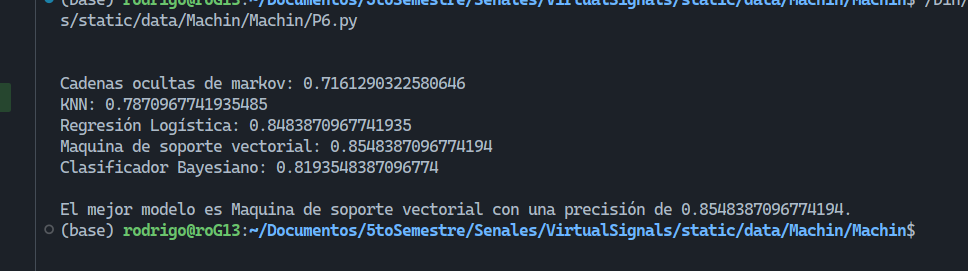
\includegraphics[width=1\textwidth]{fotomarkov.png} % Cambia 'ruta/al/archivo.jpg' por la ruta de tu imagen
	\caption{Resultados} % El texto del pie de imagen
	\label{fig:imagen2} % Etiqueta para referenciar la imagen
\end{figure}


\clearpage
\section*{Codigo completo}
\begin{lstlisting}[language=Python]


import pandas as pd
import numpy as np
from sklearn.preprocessing import StandardScaler
from sklearn.neighbors import KNeighborsClassifier
from sklearn.linear_model import LogisticRegression
from sklearn.svm import SVC
from sklearn.naive_bayes import GaussianNB
from sklearn.metrics import accuracy_score
from sklearn.base import clone
from sklearn.pipeline import Pipeline
from hmmlearn import hmm
from sklearn.preprocessing import LabelEncoder
from sklearn.model_selection import train_test_split, KFold

def cargar_datos(ruta_csv):
data = pd.read_csv(ruta_csv, header=None)
X = data.iloc[:, :-1].values
y = data.iloc[:, -1].values
return X, y

def cargar_datos_markov(filename):
columns = ['', '', '', '', '', '', '']
data = pd.read_csv(filename, header=None, names=columns)
label_encoder = LabelEncoder()
data['label'] = label_encoder.fit_transform(data['label'])
return data, label_encoder


def separar_datos_markov(data):
X = data[['', '', '', '', '', '']]
y = data['label']
return train_test_split(X, y, test_size=0.3, random_state=42)

def entrenar_markov(X_train, y_train):
hmms = {}
for label in y_train.unique():
model = hmm.GaussianHMM(n_components=4, covariance_type="diag", n_iter=100)
model.fit(X_train[y_train == label])
hmms[label] = model
return hmms

def clasificar_markov(X_test, hmms) -> list:
predictions = []
for index, row in X_test.iterrows():
max_score = float('-inf')
best_label = None
for label, model in hmms.items():
score = model.score(row.to_frame().T)
if score > max_score:
max_score = score
best_label = label
predictions.append(best_label)
return predictions

def evaluar_markov(predictions, y_test):
return sum(predictions == y_test) / len(y_test)

def validacion_cruzada_kfold(data, k):
kf = KFold(n_splits=k, shuffle=True, random_state=42)
scores = []

for train_index, test_index in kf.split(data):
X_train, X_test = data.iloc[train_index], data.iloc[test_index]
y_train, y_test = X_train['label'], X_test['label']
X_train = X_train.drop('label', axis=1)
X_test = X_test.drop('label', axis=1)

hmms = entrenar_markov(X_train, y_train)
predictions = clasificar_markov(X_test, hmms)
score = evaluar_markov(predictions, y_test)
scores.append(score)

return sum(scores) / len(scores)

def puntaje_markov(archivo):
data, label_encoder = cargar_datos_markov(archivo)
accuracy_promedio = validacion_cruzada_kfold(data, 5)
return accuracy_promedio

def k_fold_cross_validation(X, y, k, modelo):
fold_size = len(X) // k
indices = np.arange(len(X))
np.random.shuffle(indices)
scores = []

for fold in range(k):
test_indices = indices[fold * fold_size : (fold + 1) * fold_size]
train_indices = np.setdiff1d(indices, test_indices)


X_train, X_test = X[train_indices], X[test_indices]
y_train, y_test = y[train_indices], y[test_indices]


modelo_clonado = clone(modelo)
modelo_clonado.fit(X_train, y_train)


y_pred = modelo_clonado.predict(X_test)
score = accuracy_score(y_test, y_pred)
scores.append(score)

return scores

def evaluar_con_kfold_manual(X, y, k=5):
modelos = {
	'KNN': Pipeline([('scaler', StandardScaler()), ('classifier', KNeighborsClassifier(n_neighbors=5))]),
	'Regresion Logistica': Pipeline([('scaler', StandardScaler()), ('classifier', LogisticRegression(random_state=42))]),
	'Maquina de soporte vectorial': Pipeline([('scaler', StandardScaler()), ('classifier', SVC(kernel='linear', random_state=42))]),
	'Clasificador Bayesiano': Pipeline([('scaler', StandardScaler()), ('classifier', GaussianNB())])
}

resultados = dict()
resultados['Cadenas ocultas de markov'] =  puntaje_markov('dataset.csv')
print(f"\n\nCadenas ocultas de markov: {resultados['Cadenas ocultas de markov']}")

for nombre, modelo in modelos.items():
scores = k_fold_cross_validation(X, y, k, modelo)
resultados[nombre] = scores
print(f"{nombre}: {np.mean(scores)}")
mejor_modelo = max(resultados, key=lambda nombre: np.mean(resultados[nombre]))

print(f"\nEl mejor modelo es {mejor_modelo} con una precision de {np.mean(resultados[mejor_modelo])}.")




def main(ruta_csv):
X, y = cargar_datos(ruta_csv)
evaluar_con_kfold_manual(X, y)

if __name__ == "__main__":
main("dataset.csv")




\end{lstlisting}

\newpage
\section*{Conclusión}
Las cadenas de Markov son una forma de modelado estocástico que se utiliza para predecir la probabilidad de diferentes estados en un sistema. Un aspecto fundamental es que la probabilidad de transición a un estado futuro depende únicamente del estado actual, no del historial de estados. Esto se conoce como la propiedad de "falta de memoria".\vspace{1cm}

Los modelos de Markov, como cualquier modelo predictivo, pueden necesitar ajustes y actualizaciones a medida que se dispone de nuevos datos o cuando cambian las condiciones del sistema que están modelando.\vspace{1cm}

Diseñar un modelo predictivo con cadenas de Markov es un proceso que involucra una comprensión clara del problema, una cuidadosa recopilación y preparación de datos, la estimación precisa de probabilidades de transición, y una validación y mantenimiento continuos del modelo. Su aplicación puede ser extremadamente valiosa en una variedad de campos, desde la meteorología hasta la economía y más allá.

\end{document}
